%---------- Inleiding ---------------------------------------------------------

% TODO: Is dit voorstel gebaseerd op een paper van Research Methods die je
% vorig jaar hebt ingediend? Heb je daarbij eventueel samengewerkt met een
% andere student?
% Zo ja, haal dan de tekst hieronder uit commentaar en pas aan.

%\paragraph{Opmerking}

% Dit voorstel is gebaseerd op het onderzoeksvoorstel dat werd geschreven in het
% kader van het vak Research Methods dat ik (vorig/dit) academiejaar heb
% uitgewerkt (met medesturent VOORNAAM NAAM als mede-auteur).
% 

\section{Inleiding}%
\label{sec:inleiding}

Twintig jaar geleden was er nauwelijks sprake van Belgische wijnbouw. De laatste jaren is deze sector echter uitgegroeid tot een productieve pijler binnen onze landbouw. Volgens \textcite{FODEconomie2024} werd er in 2023 meer dan 3,4 miljoen liter wijn geproduceerd, en die groei zet zich voort. Ten opzichte van het voorgaande jaar steeg de productie met bijna dertien procent, terwijl het aantal hectaren met elf procent toenam. Daarom krijgt deze sector aandacht binnen het \textit{Flanders AI Research Programme} (FAIR). FAIR is een consortium van onderzoeksgroepen aan Vlaamse universiteiten en onderzoekscentra, gericht op AI-onderzoek in diverse Vlaamse sectoren. Het Instituut voor Landbouw-, Visserij- en Voedingsonderzoek (ILVO) is een van deze centra. Samen met UAntwerpen werken zij aan een usecase om taken autonoom uit te voeren in wijngaarden met behulp van AI, waaronder het monitoren van de druivenkwaliteit. 

Voor dit doel wordt een reinforcement learning (RL)-algoritme ontwikkeld dat op een kleine landbouwrobot wordt geïmplementeerd. De robot heeft een arm en sensoren om druiven te meten. Om een taak autonoom uit te voeren zijn drie controlesystemen nodig: navigatiecontrole, actuatorcontrole en taakcontrole. Het RL-model moet deze controllers samenvoegen tot één geïntegreerde controller zodat de robot zelfstandig beslissingen kan nemen, afhankelijk van de situatie.

Opdat het RL-model een goede beslissing kan nemen, moet duidelijke omgevingsinformatie worden aangereikt. Er is besloten dit te doen in de vorm van een lokale 2D-kaart van de omgeving, opgesteld met Lidar- en camerasensordata. Een mogelijke methode hiervoor is het inkleuren van gekalibreerde puntenwolken met informatie uit gesegmenteerde beelden, om deze vervolgens te projecteren op een vlak parallel aan het grondvlak. Deze bachelorproef draagt bij aan de interpretatie van camerabeelden door semantische segmentatie te realiseren.

Het semantische segmentatiemodel moet in realtime de druivenranken en -trossen kunnen segmenteren. Dergelijke modellen vereisen veel rekenkracht en geheugen. Bovendien presteren ze vaak minder goed in landbouw, omdat hun architectuur niet afgestemd is op de complexiteit van natuurlijke omgevingen en vanwege het beperkte aantal (gelabelde) datasets. Dit leidt tot de hoofdonderzoeksvraag: \emph{'Hoe kan een deep learning model worden toegepast voor realtime segmentatie van druivenranken en -trossen in wijngaarden, en hoe draagt gesynthetiseerde data bij aan de generalisatie?'}

De volgende deelvragen worden in deze bachelorproef behandeld:
\begin{itemize}
    \setlength{\itemsep}{0pt}
    \setlength{\parskip}{0pt}
    \item Wat zijn de kenmerken van een wijngaard?
    \item Welke uitdagingen ondervinden segmentatiemodellen bij toepassing in de landbouw?
    \item Welk model is geschikt voor druivenranken en -trossen?
    \item Op welke manier dient de synthetische data te worden samengesteld om het segmentatiemodel beter te trainen?
    \item Hoe kan modeloptimalisatie plaatsvinden om segmentatie in realtime mogelijk te maken?
\end{itemize}

Het eindresultaat van de bachelorproef is een \textbf{proof-of-concept} van het afgestemde segmentatiemodel voor de robot, dat gewassen in wijngaarden kan segmenteren. De prestaties van het model en de evaluaties binnen het onderzoek tonen aan of synthetische data de generalisatie heeft verbeterd.

%---------- Stand van zaken ---------------------------------------------------

\section{Literatuurstudie}%
\label{sec:literatuurstudie}

\subsection{Uitdagingen van segmentatie binnen precisielandbouw}
Uit onderzoek van \textcite{Luo2024} blijkt dat de interesse in deep learning, en meer specifiek in semantische segmentatie, binnen de precisielandbouw groeit. Deze techniek speelt een belangrijke rol in toepassingen gebaseerd op computervisie. Ze maakt het mogelijk om objecten op pixelniveau binnen een afbeelding te classificeren en toe te wijzen aan specifieke klassen. Modellen, zoals U-Net, SegNet en DeepLab, worden tegenwoordig vaak toegepast in diverse segmentatietoepassingen. Toch blijkt segmentatie binnen complexe landbouwomgevingen nog steeds een uitdaging te zijn. De robuustheid van bestaande segmentatiemethoden voor het verwerken van complexe afbeeldingen moet namelijk verbeterd worden. Daarnaast blijft hun vermogen om te generaliseren naar ongeziene data beperkt. Een bijkomend obstakel is het beperkte aantal gelabelde data, wat de training en evaluatie van nieuw ontwikkelde deep learning-modellen bemoeilijkt. Segmentatiemethoden die de dataset uitbreiden met augmentatie, zoals het gebruik van synthetische data, stellen deep learning-methoden in staat hun segmentatiemogelijkheden te verbeteren.

Onderzoek van \textcite{Charisis2024} bevestigt dat instantiesegmentatie dezelfde uitdagingen ervaart binnen de precisielandbouw. Zij voegen toe dat er universele prestatiemaatstaven ontbreken, waardoor modelvergelijkingen vaak afhankelijk zijn van onderzoeksspecifieke criteria. Verder zorgt de beperkte beschikbaarheid van open-source semi-automatische labeltools voor tijdsintensieve manuele annotatie van de datasets. Ten slotte vormt de praktische toepassing van het theoretische model in het veld vaak een extra uitdaging. Ondanks deze huidige knelpunten neemt de ontwikkeling van deep learning-gebaseerde segmentatie binnen de precisielandbouw snel toe. Er wordt verwacht dat deze technologie de komende jaren een aanzienlijke impact zal hebben.

\subsection{Dataset augmentatie met synthetische data}
Zoals eerder vermeld kan synthetische data bijdragen aan de uitbreiding en verbetering van bestaande datasets om semantische segmentatiemodellen te trainen. \textcite{Anderson2022} onderzochten het effect van synthetische data op de kwaliteit van datasets. Deze data werd gegenereerd op basis van CAD-productiemodellen, met als doel echte auto's te segmenteren. Uit de resultaten bleek dat modellen die uitsluitend met synthetische data getraind werden, een lage mean Intersection over Union (mIoU) hadden op de echte validatiedata. Door echter een klein aantal echte afbeeldingen toe te voegen aan de synthetische dataset, verbeterde de accuraatheid aanzienlijk. Bovendien presteerden de gebruikte modellen (U-net en Double-U-net) beter wanneer hun dataset werd uitgebreid met synthetische data, in vergelijking met modellen die enkel getraind werden op echte data.

\textcite{Anderson2022} stellen ook dat synthetische data het mogelijk maakt om sneller grote hoeveelheden trainingsdata te genereren. Daarbovenop wordt de annotatie van deze data automatisch uitgevoerd, waardoor tijd en kosten worden bespaard. Verder kunnen verschillende aspecten van de afbeeldingen eenvoudig worden aangepast, zoals de omgeving, lichtinval, enzovoort. Deze flexibiliteit is bijzonder waardevol in landbouwtoepassingen, waar onderzoekers verschillende weersomstandigheden en groeifases actief in de datasets moeten opnemen.

\subsection{Modeloptimalisatie}
\textcite{LopezGonzalez2024} stellen dat de toenemende rekencapaciteit van computers heeft geleid tot een trend waarbij convolutionele neurale netwerken (CNN’s) steeds groter en complexer worden. Dit veroorzaakt een sterke toename in het aantal parameters en berekeningen. Zulke netwerken zijn daardoor lastig te gebruiken op apparaten met beperkte middelen, zoals boordcomputers van autonome voertuigen. Om deze modellen te verkleinen zonder nauwkeurigheid te verliezen, is het essentieel om goed geteste modellen te combineren met compressietechnieken.

\textcite{Denil2013} merkten op dat het trainen of toepassen van \textit{transfer learning} op bekende CNN-modellen vaak resulteert in een overbodig aantal feature maps, onnodige berekeningen en hoog geheugengebruik, wat de prestaties nadelig beïnvloedt.

In hun paper introduceren \textcite{LopezGonzalez2024} een reeks optimalisaties voor U-Net, SegNet en DeepLabv3+. Ze combineren geavanceerde \textit{filter pruning} met verfijnde finetuningstrategieën om irrelevante convolutionele filters te identificeren en te verwijderen met behulp van Principal Component Analysis (PCA). In combinatie met een innovatieve scoreverdelingsmethode leidt dit tot aanzienlijk compactere netwerken. Voor U-Net ontwikkelden ze een unieke \textit{layer pruning}-techniek die de impact van encoder-decoder connecties analyseert en overbodige lagen elimineert. Ze rapporteren indrukwekkende resultaten, waaronder een reductie van maximaal 98,7\% in parameters en 97,5\% in floating point operations, zonder merkbare afname in nauwkeurigheid. Hierdoor worden zowel redundantie als rekenlast beperkt, terwijl de prestaties behouden blijven.

%---------- Methodologie ------------------------------------------------------
\section{Methodologie}%
\label{sec:methodologie}

De bachelorproef doorloopt een iteratief proces en richt zich op de implementatie en verfijning van het segmentatiemodel. Het proces begint met het in kaart brengen van de variatie binnen wijngaarden, waarbij relevante kenmerken worden geïdentificeerd. Vervolgens worden camerabeelden verzameld uit echte wijngaarden en data gecapteerd uit het testveld van ILVO. Daarnaast worden gesimuleerde wijngaarden opgezet om aanvullende data te genereren.

Na de dataverzameling worden evaluatiemaatstaven bepaald om de prestaties van het model te beoordelen. De modelontwikkeling begint met het selecteren van potentiële architecturen op basis van wetenschappelijke literatuur, waarna de verzamelde data wordt voorbereid. Het gekozen model wordt eerst getraind met enkel de echte data. Daarna volgt een tweede trainingsronde, waarin eerst synthetische data en vervolgens echte data worden gebruikt om het model verder te verfijnen. Beide versies van het model worden geëvalueerd.

Binnen de iteratieve cyclus ligt de nadruk op het doorvoeren van bijsturingen op basis van de evaluatie, met als doel de prestaties te verbeteren en de sim-to-real gap te verkleinen. Dit kan onder andere inhouden dat de modelarchitectuur wordt aangepast of dat de trainingsdata wordt aangevuld. Na elke bijsturing volgt een evaluatie om de impact van de aanpassingen te meten. Tot slot wordt het model geoptimaliseerd voor realtime toepassingen, waarna een finale evaluatie plaatsvindt om de nauwkeurigheid en efficiëntie onder realtime omstandigheden te bevestigen.

In figuur \ref{fig:met} wordt het verloop visueel weergegeven.

\begin{figure}[h]
    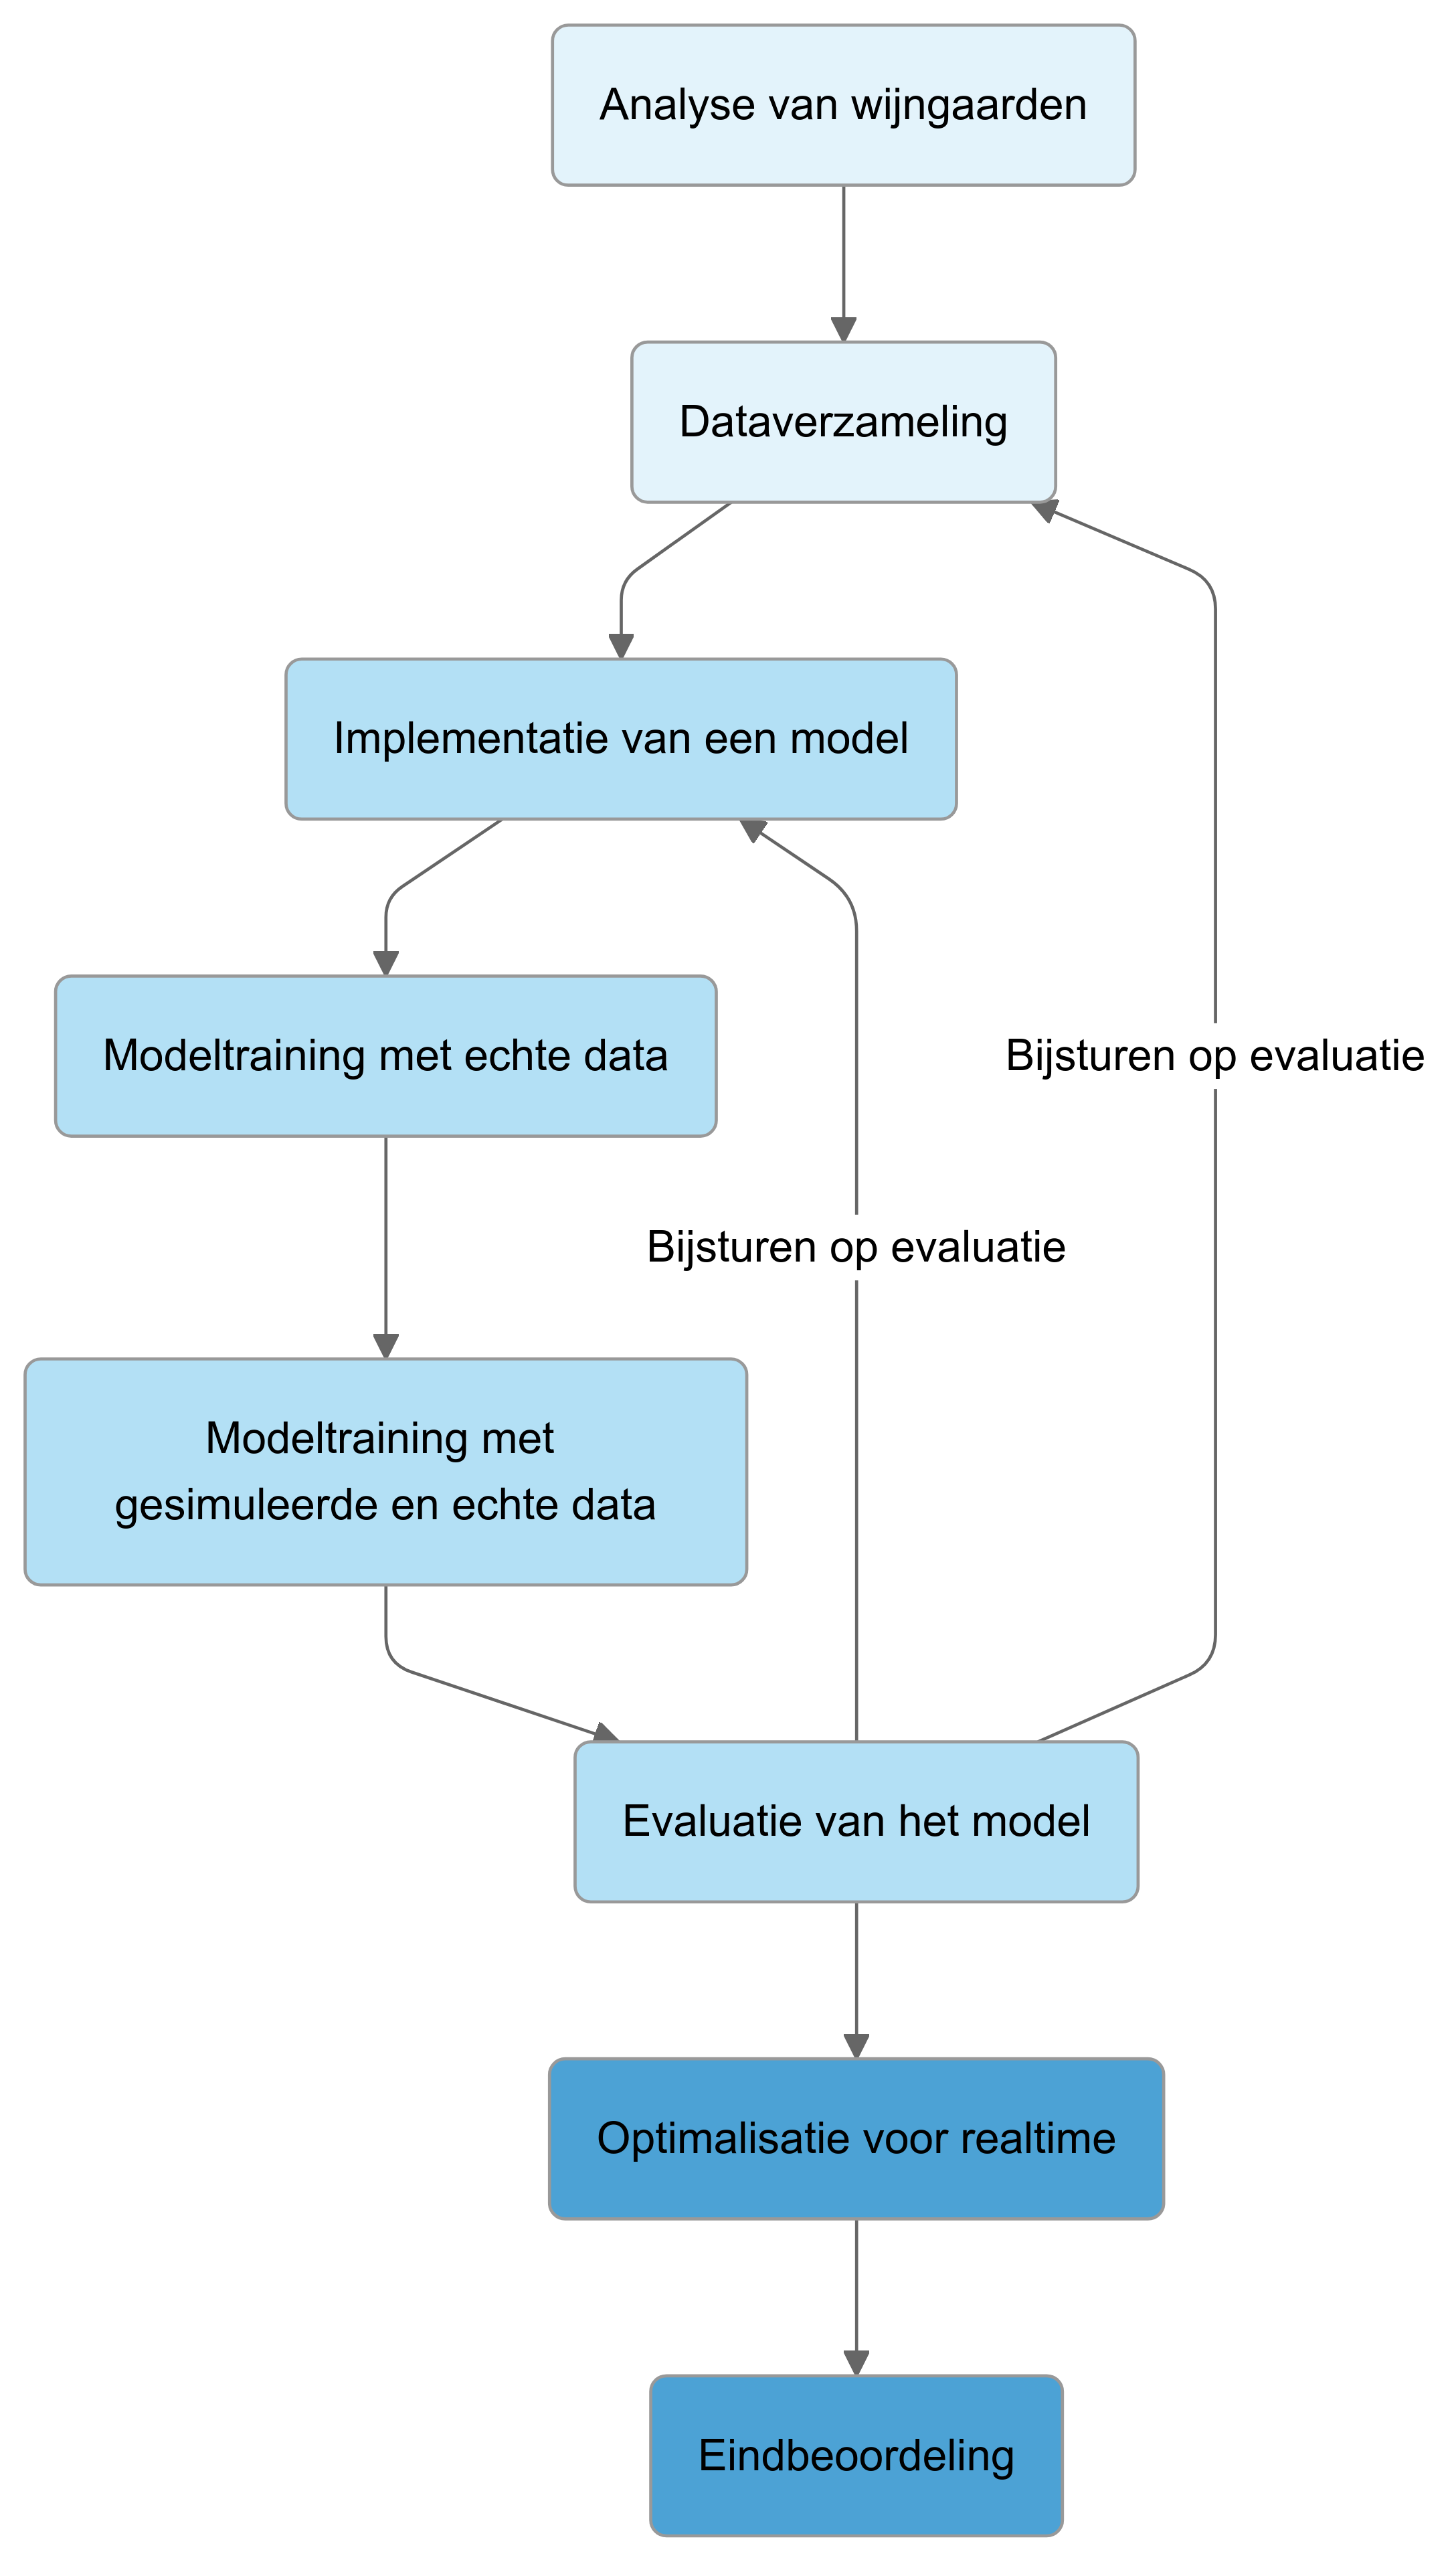
\includegraphics[width=8cm]{img/verloop.png}
    \caption{Visualisatie methodologie}
    \label{fig:met}
\end{figure}

Voor de technische uitwerking kunnen tools zoals Python, PyTorch, GitHub en Blender worden ingezet; deze lijst is mogelijks niet exhaustief of definitief.

%---------- Verwachte resultaten ----------------------------------------------
\section{Verwacht resultaat, conclusie}%
\label{sec:verwachte_resultaten}

\subsection{Segmentatiemodel}
Het onderzoek beoogt een inzetbaar segmentatiemodel te ontwikkelen dat toepasbaar is op een veldrobot voor het segmenteren van druivenplanten in camerabeelden. Het model wordt beoordeeld op nauwkeurigheid en efficiëntie. De nauwkeurigheid wordt vastgesteld door te kijken hoe goed de segmentaties van het model overeenkomen met handmatige annotaties. Belangrijke evaluatiemaatstaven hiervoor zijn Intersection over Union (IoU), de Dice-coëfficiënt, precisie, recall, de boundary F1-score, pixelnauwkeurigheid en mean Average Precision (mAP). Daarnaast wordt de efficiëntie van het model beoordeeld op inferentietijd, modelgrootte, geheugengebruik en de benodigde rekenkracht voor realtime toepassing.

\subsection{Synthetische traindata}
Er wordt verwacht dat gesynthetiseerde data een merkbaar positief effect zal hebben op de generalisatie van het model. Dit komt doordat het tekort aan echte data wordt aangevuld en een bredere variatie aan omstandigheden wordt geboden. De prestaties van het model, getraind uitsluitend met beperkte echte data, worden vergeleken met die van het model dat zowel met echte als gesynthetiseerde data is getraind. Deze manier toont aan of gesynthetiseerde data een realistische aanvulling vormt op data uit wijngaarden en kan bijdragen aan de generalisatie van het model.

\subsection{Meerwaarde}
Door segmentatie worden gewassen in de camerabeelden ingekleurd. Met behulp van gekalibreerde LIDAR-sensoren kunnen deze ingekleurde druivenranken en -trossen worden weergegeven in de gegenereerde puntwolken. Een 2D-projectie van deze 3D-datapunten vormt een kaart waarop de gewassen duidelijk zijn aangeduid. Dit biedt een visuele weergave van de gewaslocatie om het RL-model te ondersteunen bij het kiezen van acties.